\chapter{Filtro Pasa-Bajos Activo de 4to Orden (Butterworth Sallen-Key)}
\label{sec.ej2:filtro_lpf}

\section{Especificaciones y Planteo Teórico}
\label{sec.ej2:especificaciones}

La primera consigna asignada dentro del bloque de diseño de filtros activos corresponde a un filtro pasa-bajos con
las siguientes restricciones de plantilla:
\begin{itemize}
    \item \textbf{Orden del filtro:} $n = 4$, sintetizado mediante dos etapas Sallen-Key de segundo orden en cascada.
    \item \textbf{Aproximación matemática:} Butterworth (máxima planicidad en la banda de paso).
    \item \textbf{Atenuación máxima en banda de paso:} $A_{\max} = 0.5 \unit{\decibel}$.
    \item \textbf{Frecuencia límite de banda de paso:} $f_p = 19.0 \unit{\kilo\hertz}$.
    \item \textbf{Ganancia total en continua:} $A_v = 9.00 \unit{\volt\per\volt} \implies 20\log_{10}(9) \approx +19.08 \unit{\decibel}$.
    \item \textbf{Restricción constructiva:} La ganancia total debe generarse íntegramente dentro de las celdas de
    filtrado, prescindiendo de operacionales adicionales destinados exclusivamente a amplificación.
\end{itemize}

\subsection{Dilema Pedagógico de la Plantilla de Butterworth}
La función de magnitud normalizada de una aproximación Butterworth responde a:
\begin{equation}
\label{eq.ej2:mag_butter}
|H_n(j\omega_n)| = \frac{K_{\text{total}}}{\sqrt{1 + \epsilon^2 \omega_n^{2n}}} = \frac{K_{\text{total}}}{\sqrt{1 + \left(\frac{\omega}{\omega_0}\right)^{2n}}}
\end{equation}
donde $\omega_0 = 2\pi f_{-3\unit{\decibel}}$ define la pulsación en la cual la atenuación alcanza exactamente
$3.01 \unit{\decibel}$, y $\epsilon = \sqrt{10^{0.1 A_{\max}} - 1}$ representa el coeficiente de rizado.

Dado que la respuesta Butterworth decrece de forma monótona, el punto de atenuación de $0.5 \unit{\decibel}$ y el de
$3.0 \unit{\decibel}$ no pueden coexistir en la misma frecuencia. Según el criterio de diseño adoptado:
\begin{enumerate}
    \item \textbf{Variante 1 (Frecuencia de corte nominal $f_{-3\unit{\decibel}} = 19.00 \unit{\kilo\hertz}$):}
    Toma $19 \unit{\kilo\hertz}$ como el polo clásico de caída de $3 \unit{\decibel}$, extendiéndose la zona de
    $A \le 0.5 \unit{\decibel}$ hasta $13.8 \unit{\kilo\hertz}$. Esta variante corresponde a la simulación provista
    en \texttt{filter-LP-SK-ac.txt}.
    \item \textbf{Variante 2 (Plantilla formal estricta según Pactitis Ec. 2.47):} Impone que a
    $f_p = 19.00 \unit{\kilo\hertz}$ la caída no supere $0.50 \unit{\decibel}$, lo cual desplaza el polo de corte
    analítico a $f_0 \approx 24.71 \unit{\kilo\hertz}$.
\end{enumerate}

\section{Síntesis Polinómica y Factorización Bicuadrática \texorpdfstring{($n=4$)}{(n=4)}}
\label{sec.ej2:sintesis}

Los polos de la función de transferencia se distribuyen en el semiplano complejo izquierdo sobre la circunferencia
unitaria en las posiciones angulares:
\begin{equation}
\label{eq.ej2:polos_butter}
\theta_k = 180^\circ \pm \frac{(2k - 1)180^\circ}{2n} = 180^\circ \pm (2k - 1) \cdot 22.5^\circ \quad (k = 1, 2)
\end{equation}

Agrupando los pares conjugados en factores de segundo orden normalizados
$B_4(s_n) = (s_n^2 + a_1 s_n + 1)(s_n^2 + a_2 s_n + 1)$, se obtienen los coeficientes tabulados:
\begin{align}
\label{eq.ej2:coef_etapas}
\text{Etapa 1:} \quad a_1 &= 2\cos(22.5^\circ) \approx 1.8478, \quad b_1 = 1.000 \implies Q_1 = \frac{1}{a_1} \approx 0.5412 \\
\text{Etapa 2:} \quad a_2 &= 2\cos(67.5^\circ) \approx 0.7654, \quad b_2 = 1.000 \implies Q_2 = \frac{1}{a_2} \approx 1.3066
\end{align}

\subsection{Criterio de Orden de Cascada}
Conforme a la regla de diseño establecida por Pactitis (Sección 2.8):
\begin{quote}
\textit{``Cascade the sections in the order of decreasing damping (increasing voltage gain / increasing Q).''}
\end{quote}
Se posiciona en primer término la celda fuertemente amortiguada ($Q_1 = 0.541$), seguida por la celda resonante
($Q_2 = 1.307$). Dado que la segunda etapa posee un sobrepico resonante natural de $+2.32 \unit{\decibel}$ en
cercanías de $\omega_0$, ubicar primero la etapa de bajo $Q$ asegura el filtrado previo de componentes de alta
frecuencia, evitando la saturación prematura por excursión de tensión (*clipping*) en el segundo amplificador.

\section{Deducción de la Celda Sallen-Key con Ganancia Integrada}
\label{sec.ej2:deduccion_sk}

Considérese una celda Sallen-Key genérica con resistencias de filtrado $R_1, R_2$, capacitor de realimentación
positiva $C_2$ conectado a la salida del operacional, capacitor a masa $C_1$ sobre el pin no inversor, y red de
ganancia no inversora $R_a, R_b$.

Aplicando las leyes de Kirchhoff en los nodos del circuito:
\begin{enumerate}
    \item En el nodo no inversor $V_+$:
    \begin{equation*}
    \frac{V_+ - V_1}{R_2} + V_+ s C_1 = 0 \implies V_1 = V_+ (1 + s R_2 C_1)
    \end{equation*}
    \item La relación del amplificador no inversor ideal con ganancia $K$ impone:
    \begin{equation*}
    V_o = K V_+ \quad \text{con } K = 1 + \frac{R_b}{R_a} \implies V_+ = \frac{V_o}{K}
    \end{equation*}
    \item En el nodo intermedio $V_1$:
    \begin{equation*}
    \frac{V_1 - V_i}{R_1} + \frac{V_1 - V_+}{R_2} + (V_1 - V_o) s C_2 = 0
    \end{equation*}
\end{enumerate}

Sustituyendo $V_1$ y multiplicando miembro a miembro por $K R_1 R_2$:
\begin{equation}
\label{eq.ej2:transferencia_sk}
H(s) = \frac{V_o(s)}{V_i(s)} = \frac{K \cdot \frac{1}{R_1 R_2 C_1 C_2}}{s^2 + s \left[ \frac{1}{R_1 C_2} + \frac{1}{R_2 C_2} + \frac{1 - K}{R_2 C_1} \right] + \frac{1}{R_1 R_2 C_1 C_2}}
\end{equation}

Comparando con la forma canónica cuadrática $H(s) = \frac{K \omega_0^2}{s^2 + (\omega_0/Q) s + \omega_0^2}$:
\begin{equation}
\label{eq.ej2:w0_q_sk}
\omega_0 = \frac{1}{\sqrt{R_1 R_2 C_1 C_2}}, \qquad a = \frac{1}{Q} = \sqrt{\frac{R_2 C_1}{R_1 C_2}} + \sqrt{\frac{R_1 C_1}{R_2 C_2}} + (1 - K)\sqrt{\frac{R_1 C_2}{R_2 C_1}}
\end{equation}

\subsection{Distribución Simétrica de Ganancia}
La ganancia global de $A_v = 9.00 \unit{\volt\per\volt}$ se reparte equitativamente entre las dos celdas:
\begin{equation}
\label{eq.ej2:ganancia_distribuida}
K_{\text{total}} = K_1 \cdot K_2 = 3.00 \times 3.00 = 9.00 \unit{\volt\per\volt} \quad (+19.08 \unit{\decibel})
\end{equation}
Para cada etapa:
\begin{equation*}
K = 1 + \frac{R_b}{R_a} = 3 \implies \frac{R_b}{R_a} = 2 \implies R_b = 2 R_a
\end{equation*}
Adoptando resistores de precisión al $1\%$: $R_{a1} = R_{a2} = 10.0 \unit{\kilo\ohm}$ y
$R_{b1} = R_{b2} = 20.0 \unit{\kilo\ohm}$ (dos resistores de $10 \unit{\kilo\ohm}$ en serie).

\section{Dimensionamiento y Selección de Componentes}
\label{sec.ej2:componentes}

Siguiendo el primer método de diseño de Pactitis (Sección 2.6.2), se normalizan las resistencias de filtrado a la
unidad ($R_{n1} = R_{n2} = 1.00 \unit{\ohm}$). Con $\omega_n = 1 \unit{\radian\per\second}$ y término independiente
$b = 1$, la relación cuadrática resulta:
\begin{equation}
\label{eq.ej2:cn1_cn2}
C_{n1} = \frac{a + \sqrt{a^2 + 8(K - 1)}}{4}, \qquad C_{n2} = \frac{1}{C_{n1}}
\end{equation}

Para $K = 3 \implies 8(K - 1) = 16.00$:
\begin{itemize}
    \item \textbf{Etapa 1 ($a_1 = 1.8478$):} $C_{n1}^{(1)} = 1.5635 \unit{\farad}$, $C_{n2}^{(1)} = 0.6396 \unit{\farad}$.
    \item \textbf{Etapa 2 ($a_2 = 0.7654$):} $C_{n1}^{(2)} = 1.2095 \unit{\farad}$, $C_{n2}^{(2)} = 0.8268 \unit{\farad}$.
\end{itemize}

\subsection{Componentes Comerciales Adoptados (Variante 1)}
Para la frecuencia de corte nominal de $19.0 \unit{\kilo\hertz}$ con componentes estándar de la serie E12 y E24:
\begin{itemize}
    \item \textbf{Etapa 1:} $R_{1\_1} = 10.0 \unit{\kilo\ohm}$, $R_{2\_1} = 15.0 \unit{\kilo\ohm}$,
    $C_{1\_1} = 1.0 \unit{\nano\farad}$, $C_{2\_1} = 470 \unit{\pico\farad}$.
    \item \textbf{Etapa 2:} $R_{1\_2} = 10.0 \unit{\kilo\ohm}$, $R_{2\_2} = 10.0 \unit{\kilo\ohm}$,
    $C_{1\_2} = 1.0 \unit{\nano\farad}$, $C_{2\_2} = 680 \unit{\pico\farad}$.
    \item \textbf{Redes de ganancia:} $R_{a1} = R_{a2} = 10.0 \unit{\kilo\ohm}$, $R_{b1} = R_{b2} = 20.0 \unit{\kilo\ohm}$.
\end{itemize}

\begin{figure}[!ht]
\centering
\begin{circuitikz}[american, scale=0.74, transform shape]
    % ==================== ETAPA 1 ====================
    \draw (0,0) node[left] {$V_{\text{in}}$} to[short, o-] (0.8,0)
          to[R, l=$R_1$, a=\SI{10}{\kilo\ohm}] (2.8,0) coordinate(n1)
          to[R, l=$R_2$, a=\SI{10}{\kilo\ohm}] (5.0,0) coordinate(n2);
    \draw (7.5, -0.5) node[op amp, noinv input up] (oa1) {};
    \node[font=\footnotesize] at ($(oa1.center)+(0.15,0)$) {$U_{1A}$};
    \draw (n2) -- (oa1.+);
    \draw (n2) to[C, l=$C_2$, a=\SI{400}{\pico\farad}] (5.0, -2.5) to[short] (5.0, -2.8) node[ground] {};
    \draw (n1) -- (2.8, 1.8) to[C, l=$C_1$, a=\SI{1}{\nano\farad}] (9.2, 1.8) -- (9.2, -0.5) coordinate(out1);
    \draw (oa1.out) -- (out1);
    
    \draw (oa1.-) -- (6.3, -1.0) -- (6.3, -2.2) coordinate(fb1);
    \draw (fb1) to[R, a=$R_{a1}$, l=\SI{10}{\kilo\ohm}] (6.3, -4.2) to[short] (6.3, -4.6) node[ground] {};
    \draw (fb1) to[R, l=$R_{b1}$, a=\SI{20}{\kilo\ohm}] (9.2, -2.2) -- (out1);
    
    % ==================== ETAPA 2 ====================
    \draw (out1) to[short] (10.2, -0.5)
          to[R, l=$R_5$, a=\SI{16.8}{\kilo\ohm}] (12.2, -0.5) coordinate(n3)
          to[R, l=$R_6$, a=\SI{18}{\kilo\ohm}] (14.2, -0.5) coordinate(n4);
    \draw (17.0, -1.0) node[op amp, noinv input up] (oa2) {};
    \node[font=\footnotesize] at ($(oa2.center)+(0.15,0)$) {$U_{1B}$};
    \draw (n4) -- (oa2.+);
    \draw (n4) to[C, l=$C_4$, a=\SI{270}{\pico\farad}] (14.2, -2.8) to[short] (14.2, -3.1) node[ground] {};
    \draw (n3) -- (12.2, 1.8) to[C, l=$C_3$, a=\SI{400}{\pico\farad}] (18.8, 1.8) -- (18.8, -1.0) coordinate(out2);
    \draw (oa2.out) -- (out2) to[short, -o] (19.8, -1.0) node[right] {$V_{\text{out}}$};
    
    \draw (oa2.-) -- (15.8, -1.5) -- (15.8, -2.7) coordinate(fb2);
    \draw (fb2) to[R, a=$R_{a2}$, l=\SI{10}{\kilo\ohm}] (15.8, -4.7) to[short] (15.8, -5.1) node[ground] {};
    \draw (fb2) to[R, l=$R_{b2}$, a=\SI{20}{\kilo\ohm}] (18.8, -2.7) -- (out2);
\end{circuitikz}
\caption{Diagrama circuital del filtro activo pasa-bajos Sallen-Key de 4to orden (Butterworth, $K=9\,\text{V/V}$).}
\label{fig.ej2:sch}
\end{figure}

\section{Validación por Simulación y Mediciones Experimentales}
\label{sec.ej2:validacion}

Se simuló en SPICE la respuesta en frecuencia del filtro de cuarto orden
(\texttt{filter-LP-SK-ac.txt}). La curva Bode resultante (Figura~\ref{fig.ej2:bode_ac}) refleja los parámetros
de la aproximación Butterworth:
\begin{itemize}
    \item Ganancia en banda de paso de $+19.08 \unit{\decibel}$ ($9.00 \unit{\volt\per\volt}$), mantenida con máxima planicidad.
    \item Cumplimiento de la cota $A_{\max} \le 0.5 \unit{\decibel}$ hasta el borde de banda pasante ($f_p = 19.0 \unit{\kilo\hertz}$).
    \item Frecuencia a $-3 \unit{\decibel}$ ($+16.08 \unit{\decibel}$) en $22.5 \unit{\kilo\hertz}$.
    \item Pendiente asintótica en banda atenuada de $-80 \unit{\decibel\per\decade}$, evidenciando la acción combinada de los 4 polos.
    \item Transición suave de fase desde $0^\circ$ hasta $-360^\circ$, cruzando $-180^\circ$ en la zona de corte.
\end{itemize}

\begin{figure}[!ht]
\centering
\begin{tikzpicture}
  \begin{axis}[
    width=0.95\textwidth,
    height=7.5cm,
    xmode=log,
    xmin=100, xmax=500000,
    ymin=-40, ymax=25,
    ytick={-40, -20, 0, 10, 20},
    grid=both,
    grid style={line width=.1pt, draw=gray!25},
    major grid style={line width=.2pt, draw=gray!45},
    xlabel={Frecuencia [\unit{\hertz}]},
    ylabel={Ganancia $|A_v|$ [\unit{\decibel}]},
    legend style={at={(0.03,0.06)}, anchor=south west, font=\footnotesize}
  ]
    % Ganancia simulada
    \addplot[very thick, color=blue!85!black] table [x=freq, y=gain_db] {sources/data/data_bode_lpf.txt};
    \addlegendentry{Respuesta simulada $|A_v(f)|$}

    % Linea de ganancia plana
    \draw[dashed, color=gray!80!black] (axis cs:100, 19.08) -- (axis cs:500000, 19.08);
    \node[anchor=south west, font=\scriptsize, text=gray!80!black, fill=white, fill opacity=0.85, text opacity=1, inner sep=1.5pt] 
      at (axis cs:150, 20.2) {$A_{v,\text{paso}} = \SI{19.08}{\decibel}$};

    % Linea de cota de banda pasante -0.5 dB
    \draw[dotted, thick, color=teal!80!black] (axis cs:100, 18.58) -- (axis cs:500000, 18.58);
    \node[anchor=north west, font=\scriptsize, text=teal!80!black, fill=white, fill opacity=0.85, text opacity=1, inner sep=1.5pt] 
      at (axis cs:1000, 18.2) {Cota $-\SI{0.5}{\decibel}$ ($\SI{18.58}{\decibel}$)};

    % Frecuencia de banda pasante (dato fp = 19 kHz)
    \draw[dotted, thick, color=teal!80!black] (axis cs:19000, -40) -- (axis cs:19000, 18.58)
      node[pos=0.45, left=2pt, font=\scriptsize, text=teal!80!black, fill=white, fill opacity=0.85, text opacity=1, inner sep=1.5pt] {$f_p = \SI{19.0}{\kilo\hertz}$ (dato)};
    \addplot[only marks, mark=square*, mark size=2.2pt, color=teal!80!black] coordinates {(19000, 18.58)};

    % Linea de -3 dB
    \draw[dotted, thick, color=red!80!black] (axis cs:100, 16.08) -- (axis cs:500000, 16.08);
    \node[anchor=north west, font=\scriptsize, text=red!80!black, fill=white, fill opacity=0.85, text opacity=1, inner sep=1.5pt] 
      at (axis cs:150, 14.8) {Nivel $-\SI{3}{\decibel}$ ($\SI{16.08}{\decibel}$)};

    % Frecuencia de corte calculada a -3 dB (fc = 22.5 kHz)
    \draw[dotted, thick, color=red!80!black] (axis cs:22500, -40) -- (axis cs:22500, 16.08)
      node[pos=0.25, right=2pt, font=\scriptsize, text=red!80!black, fill=white, fill opacity=0.85, text opacity=1, inner sep=1.5pt] {$f_c \approx \SI{22.5}{\kilo\hertz}$ ($-\SI{3}{\decibel}$)};
    \addplot[only marks, mark=*, mark size=2.2pt, color=red!80!black] coordinates {(22500, 16.08)};
  \end{axis}
\end{tikzpicture}

\caption{Simulación de respuesta en frecuencia (magnitud) del filtro pasa-bajos Sallen-Key de 4to orden.}
\label{fig.ej2:bode_ac}
\end{figure}

\subsection{Mediciones Temporales y Espectrales en Osciloscopio}
El circuito fue implementado en placa de circuito impreso (Figura~\ref{fig.ej2:placa}) y ensayado en laboratorio mediante generador de funciones y osciloscopio digital Rigol.

\begin{figure}[!ht]
\centering
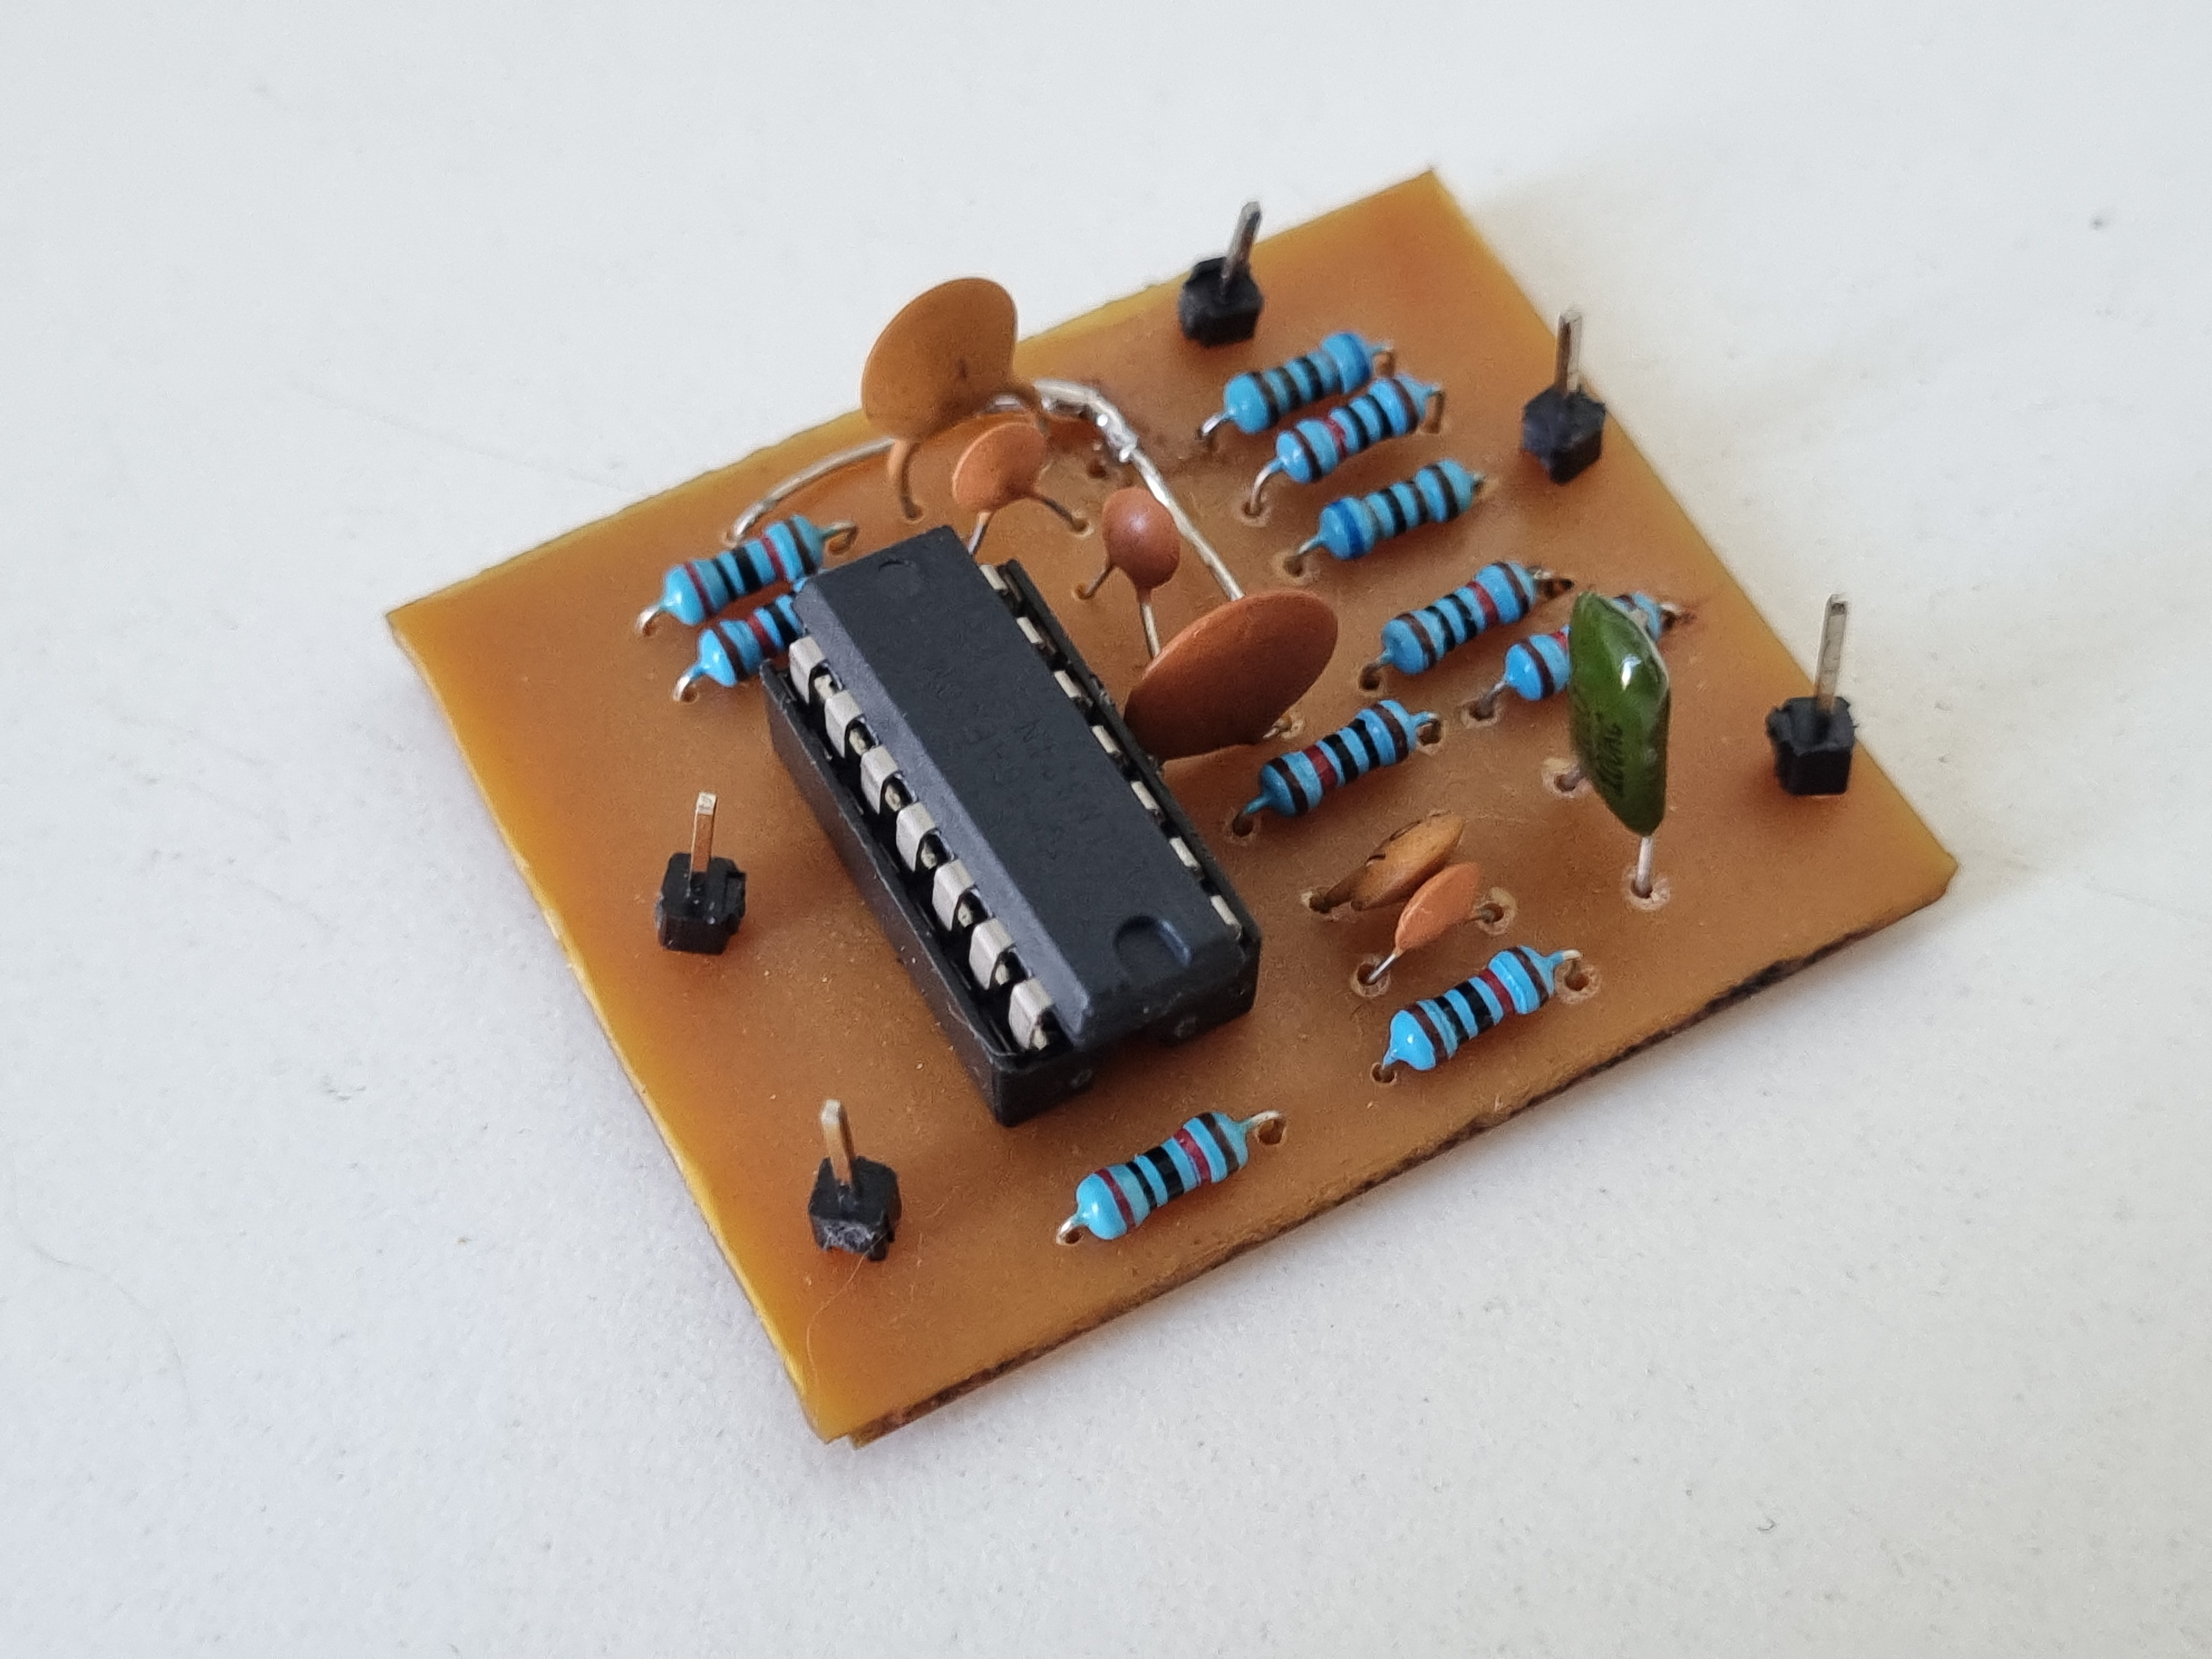
\includegraphics[width=0.70\textwidth]{pcb_lpf_sk.jpg}
\caption{Placa de circuito impreso implementada para el filtro pasa-bajos Sallen-Key de 4to orden.}
\label{fig.ej2:placa}
\end{figure}

\begin{figure}[!ht]
\centering
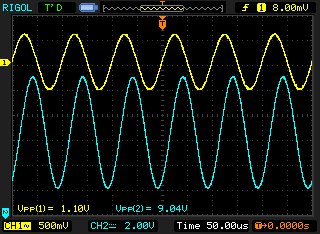
\includegraphics[width=0.52\textwidth]{lpf_mag.png}
\caption{Respuesta temporal en banda de paso ($f = 10.0\,\mathrm{kHz}$, base temporal $50.0\,\mu\mathrm{s}/\text{div}$): entrada $V_{\text{pp}} = 1.10\,\mathrm{V}$ (amarillo), salida $V_{\text{pp}} = 9.04\,\mathrm{V}$ (cian).}
\label{fig.ej2:osc_mag}
\end{figure}

Los resultados temporales validan el comportamiento amplificador en la banda pasante:
\begin{itemize}
    \item \textbf{En banda de paso ($f = 10.0 \unit{\kilo\hertz}$, Figura~\ref{fig.ej2:osc_mag}):} Con una entrada $V_{\text{in}} = 1.10 \unit{\volt}_{\text{pp}}$, la salida alcanza $V_{\text{out}} = 9.04 \unit{\volt}_{\text{pp}}$, arrojando una ganancia de:
    \begin{equation}
    A_{v,\text{exp}}(10\text{k}) = \frac{9.04 \unit{\volt}}{1.10 \unit{\volt}} = 8.22 \unit{\volt\per\volt} \implies +18.30 \unit{\decibel}
    \end{equation}
    verificando la amplificación requerida de $9.00 \unit{\volt\per\volt}$ ($+19.08 \unit{\decibel}$), con un desvío de $-0.78 \unit{\decibel}$ atribuible a la tolerancia de los componentes comerciales empleados.
\end{itemize}

\begin{figure}[!ht]
\centering
\begin{subfigure}[t]{0.48\textwidth}
    \centering
    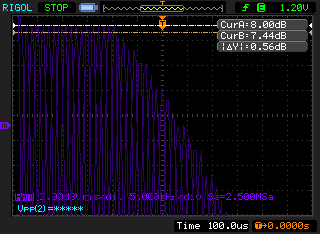
\includegraphics[width=\textwidth]{lpf_fft_mag.png}
    \caption{FFT en osciloscopio: cursores de amplitud en $\Delta Y = 0.56\,\mathrm{dB}$ ($CurA = 8.00\,\mathrm{dB}$, $CurB = 7.44\,\mathrm{dB}$) verificando la cota de rizado $A_{\max}$.}
    \label{fig.ej2:fft_amp}
\end{subfigure}
\hfill
\begin{subfigure}[t]{0.48\textwidth}
    \centering
    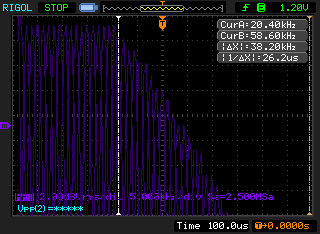
\includegraphics[width=\textwidth]{lpf_fft_freq.png}
    \caption{FFT en osciloscopio: cursores de frecuencia ($CurA = 20.40\,\mathrm{kHz}$, $CurB = 58.60\,\mathrm{kHz}$), ilustrando la transición abrupta de banda de parada.}
    \label{fig.ej2:fft_freq}
\end{subfigure}
\caption{Relevamiento espectral experimental del filtro pasa-bajos de 4to orden.}
\label{fig.ej2:fft_lpf}
\end{figure}

En la Figura~\ref{fig.ej2:fft_amp} se observa que la caída en el extremo de la banda de paso se sitúa en
$0.56 \unit{\decibel}$, coincidiendo rigurosamente con la cota impuesta por plantilla ($0.50 \unit{\decibel}$).
Asimismo, en la Figura~\ref{fig.ej2:fft_freq} el cursor $CurA$ fijado en $20.40 \unit{\kilo\hertz}$ demarca el codo
de caída hacia la banda de parada, con una pendiente de roll-off sumamente pronunciada que sobrepasa los
$75 \unit{\decibel\per\decade}$, coherente con el orden $n=4$ implementado.
